\documentclass[aspectratio=169]{beamer}

\usefonttheme{professionalfonts}


% Document metadata

\subtitle{ELEC0447 - Analysis of electric power and energy systems}
\title{Course organization and introduction}
\author[BC]{Bertrand Cornélusse}
\institute{Univeristy of Liège}
\date{\today}

% Image for the title page (use include graphics option to properly size/place it)
\titlegraphic{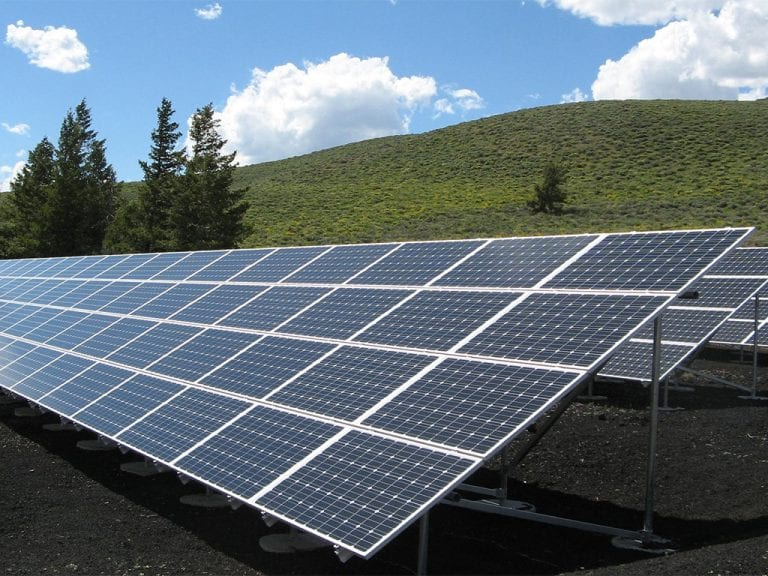
\includegraphics[height=\paperheight]{banner.jpg}}
\usetheme[titlestyle=style1]{trigon}
%\usetheme[sectionstyle=style2]{trigon}

% Define logos to use (comment if no logo)
\biglogo{uliege_faculte_sciencesappliquees_logo_rvb_pos.pdf} % Used on titlepage only
\smalllogo{} % Used on top right corner of regular frames

% ------ If you want to change the theme default colors, do it here ------
%\definecolor{tPrim}{HTML}{00843B}   % Green
%\definecolor{tSec}{HTML}{289B38}    % Green light
%\definecolor{tAccent}{HTML}{F07F3C} % Orange

% ------ Packages and definitions used for this demo. Can be removed ------
\usepackage{appendixnumberbeamer} % To use \appendix command
\pdfstringdefDisableCommands{% Fix hyperref translate warning with \appendix
\def\translate#1{#1}%
}
\usepackage{pgf-pie} % For pie charts
\usepackage{caption} % For subfigures
\usepackage{subcaption} % For subfigures
\usepackage{xspace}
\newcommand{\themename}{\textbf{\textsc{trigon}}\xspace}
\usepackage[scale=2]{ccicons} % Icons for CC-BY-SA
\usepackage{booktabs} % Better tables
\usepackage{amsmath}
\usepackage{amssymb}
\usepackage{amsfonts}
\usepackage{algorithm}
\usepackage{algpseudocodex}
\usepackage{multicol}
\usepackage{booktabs}
\usepackage{colortbl}
\usepackage{listings}
\usepackage{tikz}
\usepackage{blox}
\usepackage{calc}
%\usetikzlibrary{arrows.meta, positioning}




\newcommand{\Z}       {\mathbb{Z} }
\newcommand{\R}       {\mathbb{R} }
\newcommand{\Q}       {\mathbb{Q} }
\newcommand{\N}       {\mathbb{N} }
\newcommand{\spa}     {\text{span}}
\newcommand{\lin}     {\text{span}}
\newcommand{\inter}   {\text{int} }
\newcommand{\st}{\mathrm{s.t.}}
\definecolor{myRed}{RGB}{209,34,57} 


\lstset{
    language=Python,
    basicstyle=\ttfamily\scriptsize, % use a monospaced font at a smaller size
    numbers=left, % add line numbers on the left
    numberstyle=\tiny\color{gray}, % style for the line numbers
    frame=single, % put a frame around the code block
    showstringspaces=false, % don't show special characters for spaces in strings
    tabsize=4, % set tab size
    keywordstyle=\color{blue}\bfseries, % bold and blue keywords
    stringstyle=\color{red}, % red strings
    commentstyle=\color{green!60!black}\itshape % italic and dark green comments
}

%==============================================================================
%                               BEGIN DOCUMENT
%==============================================================================
\begin{document}


%--------------------------------------
% Create title frame
\titleframe

%--------------------------------------
% Table of contents
\begin{frame}{Overview}
  \setbeamertemplate{section in toc}[sections numbered]
  \tableofcontents[hideallsubsections]
\end{frame}

\section{Introduction}

\begin{frame}[allowframebreaks]{What is a power flow analysis?}
    Power flow (or load flow) analysis aims at determining the \textit{electrical state of an electrical power system}, when information about power generated or consumed is available at nodes of the network, and considering that the voltage level is regulated at some buses.
    
    This type of analysis is commonly used by power companies for planning and operation purposes.
    \begin{itemize}
        \item If voltage magnitude and angles were measured at all buses,
        \begin{itemize}
            \item then it would boil down to solving a set of simple linear equations.
        \end{itemize}
        \item In a similar way, mesh or nodal analysis could be used if we had a full model of the system,
        \begin{itemize}
            \item even without all voltage measurements.
        \end{itemize}
        \item But here the situation is different, because we mainly have access to \textit{power} measurements.
        \begin{itemize}
            \item The system is no more linear.
        \end{itemize}
    \end{itemize}
\end{frame}

\begin{frame}[allowframebreaks]{Power flow problem statement}
    Determine \textbf{the voltage at every bus}, assuming we have a power system composed of transmission lines connecting the following bus types:
    \begin{itemize}
        \item \textit{PQ buses} are typically loads where active and reactive power are measured
        \begin{itemize}
            \item it can also be generation where voltage is not regulated (e.g. renewable generation)
        \end{itemize}
        \item \textit{PV buses} where the active power and the voltage are specified
        \begin{itemize}
            \item these are typically generators
        \end{itemize}
        \item one \textit{slack bus} that sets the reference for the voltage magnitudes and angles (it is usually at 1 pu)
        \begin{itemize}
            \item P and Q can take any value to reach the power balance in the system.
        \end{itemize}
    \end{itemize}
    
    Branch currents and losses can be determined from the voltages (magnitudes and phases).
    
    Note: as we will see, PV buses must be swithed to PQ buses in case they reach a limit of their capability curve.
\end{frame}

\begin{frame}[allowframebreaks]{A first tiny example}
    \begin{center}
        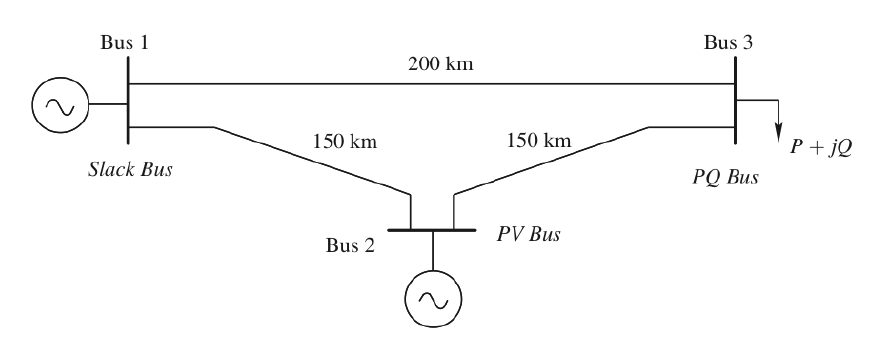
\includegraphics[width=0.8\linewidth]{images/PF_net_1.png}
    \end{center}
    \begin{columns}
        \begin{column}{0.5\linewidth}
            Buses:
            \begin{itemize}
                \item Bus 1 is the slack, with V = 1 pu
                \item Bus 2 is a PV bus, with V regulated at 1.05 pu and drawing P= 2 pu
                \item Bus 3 is a PQ bus, consumes P = 5 pu and Q = 1 pu.
            \end{itemize}
        \end{column}
        \begin{column}{0.5\linewidth}
            Lines:
            \begin{itemize}
                \item X = 0.376 Ohm/km (at 60 Hz)
                \item R = 0.037 Ohm/km
                \item Shunt susceptances are ignored (4.5e-6 S/km)
            \end{itemize}
        \end{column}
    \end{columns}
    Voltage base (3-phase): 345 kV,
    Power base (3-phase): 100 MVA
\end{frame}


\begin{frame}{Modeling the system in PandaPower}

    We will see how to describe mathematically the problem and how to solve it in the next sections.

    Usually, however, engineers use existing modeling and solution software.
    One of those, which is open source and accessible through Python scripts, is PandaPower \cite{thurner2018pandapower}. 

    \href{https://colab.research.google.com/drive/103VIzly2huoS-PjnYdbCaeBS1dunJS7H?usp=sharing}{\underline{Link to the PandaPower model}} 
    
\end{frame}

\begin{frame}[fragile, allowframebreaks]
    \frametitle{Creation of the power flow model with PandaPower}
    \begin{center}
        \lstinputlisting{pandapower_net.py}
    \end{center}
\end{frame}

\begin{frame}{Result of the tiny example using pandapower}
    
    \begin{center}
     {\scriptsize    
    \begin{tabular}{|l|r|r|r|r|}
        \hline
        & \textbf{vm\_pu} & \textbf{va\_degree} & \textbf{p\_mw} & \textbf{q\_mvar} \\
        \hline
        0 & 1.00 & 0.00 & -308.38 & 81.61 \\
        \hline
        1 & 1.05 & -2.07 & -200.00 & -266.74 \\
        \hline
        2 & 0.98 & -8.79 & 500.00 & 100.00 \\
        \hline
    \end{tabular}
     }
\end{center}

    Are there losses?
    
    Results for the lines:
    {\scriptsize
    \begin{tabular}{|l|r|r|r|r|r|r|r|r|}
        \hline
        & \textbf{p\_from\_mw} & \textbf{q\_from\_mvar} & \textbf{p\_to\_mw} & \textbf{q\_to\_mvar} & \textbf{pl\_mw} & \textbf{ql\_mvar} & \textbf{i\_from\_ka} & \textbf{i\_to\_ka} \\
        \hline
        0 & 68.99 & -110.87 & -68.20 & 118.95 & 0.80 & 8.08 & 0.22 & 0.22 \\
        \hline
        1 & 268.20 & 147.79 & -264.23 & -107.49 & 3.97 & 40.30 & 0.49 & 0.49 \\
        \hline
        2 & -235.77 & 7.49 & 239.38 & 29.26 & 3.62 & 36.75 & 0.40 & 0.40 \\
        \hline
    \end{tabular}
    }
\end{frame}

\section{The power flow equations}

\begin{frame}[allowframebreaks]{The power flow equations}
    \begin{itemize}
        \item Let $\mathcal{N}$ be the set of buses of the network
        \item Some buses are interconnected by transmission lines, given by their $\pi$ models
        \item Let $\mathcolor[RGB]{00,99,00}{Y_{kG}}$ be the sum of admittances connected between node $k$ and the ground:
        \begin{itemize}
            \item the shunt admittances of the lines incident to $k$, and the admittances of the devices connected at node $k$ if any.
        \end{itemize}
        \item For two nodes $k$ and $m$, let $Z_{km}$ be the series impedance of the line connecting them and $Y_{km} = Z_{km}^{-1}$ ($Y_{km} = 0$ if there is no line)
    \end{itemize}
    
    The current injection at node $k$ is
    \begin{equation}
        \mathcolor{blue}{\bar{I}_k} = \mathcolor[RGB]{00,99,00}{Y_{kG}} \bar{V}_k + \sum_{m \in \mathcal{N} \setminus k} {(\bar{V}_k - \bar{V}_m) Y_{km}} \label{eq:bus_inj}
    \end{equation}
   
    \begin{figure}[htbp]
        \centering
        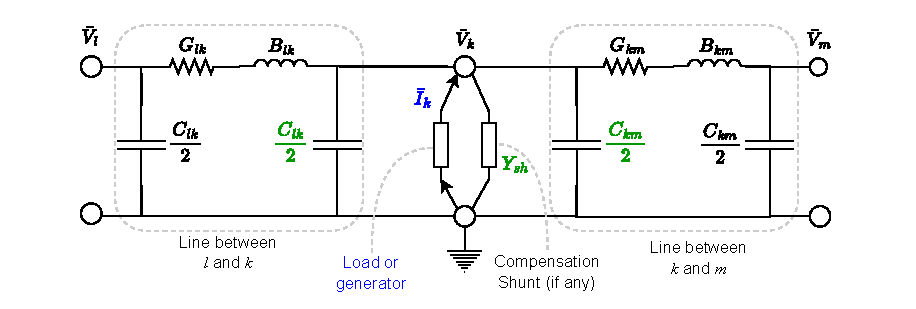
\includegraphics[width=0.8\textwidth]{images/bus_injection_model.pdf}
        \caption{Illustration of current injection at bus $k$ as a function of exchanges with neighbor buses ($l$ and $m$) and shunt compensation device. Devices and lines connected to buses $l$ and $m$ are not shown.}
        \label{fig:bus_injection}
    \end{figure}

    This last equation can be rewritten as
    $$\mathcolor{blue}{\bar{I}_k} =  \left(\mathcolor[RGB]{00,99,00}{Y_{kG}}+ \sum_{m \in \mathcal{N} \setminus k} Y_{km} \right) \bar{V}_k  - \sum_{m \in \mathcal{N} \setminus k} Y_{km} \bar{V}_m$$
    
    which highlights the possibility to write in matrix form
    \begin{equation}
        \mathbf{\bar{I}} = \mathbf{Y} \mathbf{\bar{V}} \label{eq:bus_inj_mat}
    \end{equation}
    with $\mathbf{\bar{I}}$ and $\mathbf{\bar{V}}$ the vectors of bus current injections and bus voltages, respectively.
    
    \newpage
    The \textit{admittance matrix} $\mathbf{Y}$ can be determined by inspection:
    \begin{itemize}
        \item Element $y_{kk}$ is the sum of the admittances incident to bus $k$
        \item Element $y_{km}, m \neq k$, is the opposite of the sum of the admittances connecting bus $k$ to bus $m$.
    \end{itemize}

    However, remember that we have power measurements only (and voltage magnitudes at a few PV buses). So we can derive
    \begin{equation}
        \mathbf{P} +j \mathbf{Q} = \mathbf{\bar{V}} \circ \mathbf{\bar{I}}^{\star}
        = \mathbf{\bar{V}} \circ \mathbf{Y}^{\star} \mathbf{\bar{V}}^{\star} \label{eq:pf}
    \end{equation}
    where $\mathbf{P}$ and $\mathbf{Q}$ are the vectors of active and reactive power injections, respectively, and $\circ$ denotes the elementwise product.
    
    If we develop this relation for a node $k$, we have:
    \begin{align}
        P_k &= g_{kk} V_k^2  + V_k \sum_{m \in \mathcal{N} \setminus k} V_m(g_{km} \cos\theta_{km} + b_{km} \sin\theta_{km}) = p_k(\mathbf{\bar{V}}) \label{eq:pf_P}\\
        Q_k &= -b_{kk} V_k^2 + V_k \sum_{m \in \mathcal{N} \setminus k} V_m(g_{km} \sin\theta_{km} - b_{km} \cos\theta_{km}) = q_k(\mathbf{\bar{V}}) \label{eq:pf_Q}
    \end{align}
   
    with
    \begin{itemize}
        \item $y_{km} = g_{km} + j b_{km}$
        \item $y_{kk} = g_{kk} + j b_{kk}$ 
        \item $\theta_{km} = \theta_{k} - \theta_{m}$ the phase difference between voltages at nodes $k$ and $m$
    \end{itemize}
\end{frame}

\begin{frame}[allowframebreaks]{Number of equations and unknowns}
    If there are $n$ buses in total, among which $n_{PQ}$ PQ buses, $n_{PV}$ PV buses and one slack bus, hence
    $$ n = n_{PQ} + n_{PV} + 1,$$
    then
    \begin{itemize}
        \item $\mathbf{P}$ is known for $n_{PQ} + n_{PV}$ buses (all but the slack)
        \item Elements of $\mathbf{Q}$ are known for the $n_{PQ}$ PQ buses
        \item Voltage magnitude is known at PV buses and at the slack bus
        \item Voltage angle is known at the slack bus.
    \end{itemize}
    
    \vspace{1cm}
    
    In total, there are $2n$ equations for $2n$ unknowns:
    \begin{itemize}
        \item $n-1$ voltage angles, 
        \item $n_{PQ}$ voltage magnitudes, 
        \item $n_{PV} + 1$ reactive powers, 
        \item 1 active power.
    \end{itemize} 
\end{frame}

\section{Power flow solution method}

\begin{frame}
    \frametitle{Power flow solution method}
    Let
    \begin{itemize}
        \item $\mathbf{P}^0$ be the active powers specified at the $\mathcal{N}_{PQ} \cup \mathcal{N}_{PV}$ buses
        \item $\mathbf{Q}^0$ be the reactive powers specified at the $\mathcal{N}_{PQ}$ buses.
    \end{itemize}
    
    To find $\mathbf{\bar{V}}$, we must solve
    \begin{align*}
        P_k^0 - p_k(\mathbf{\bar{V}}) &= 0, \ \forall k \in \mathcal{N}_{PQ} \cup \mathcal{N}_{PV} \\
        Q_k^0 - q_k(\mathbf{\bar{V}}) &= 0, \ \forall k \in \mathcal{N}_{PQ}
    \end{align*}
    which is a set of $2 n_{PQ} + n_{PV}$ non-linear equations.
    
    The most widespread method to solve this system is the \textit{Newton-Raphson method}.
\end{frame}


\begin{frame}[allowframebreaks]{Newton-Raphson example in 1D}
    \begin{itemize}
        \item Let's assume we want to solve $c-f(x) = 0$ with $f$ a non-linear function.
        \item We start with a first guess for $x$, $x^{(0)}$, at iteration $i=0$
        \item Then, while $|c-f(x^{(i)})| > \epsilon$:
        \begin{itemize}
            \item $x^{(i+1)} = x^{(i)} + \frac{c-f(x^{(i)})}{f'(x^{(i)})}$
            \item $i \leftarrow i + 1$
        \end{itemize}
    \end{itemize}
    
    \begin{columns}
    \begin{column}{0.55\textwidth}
    For $c=4$ and $f(x) = x^3$:
    \begin{center}
        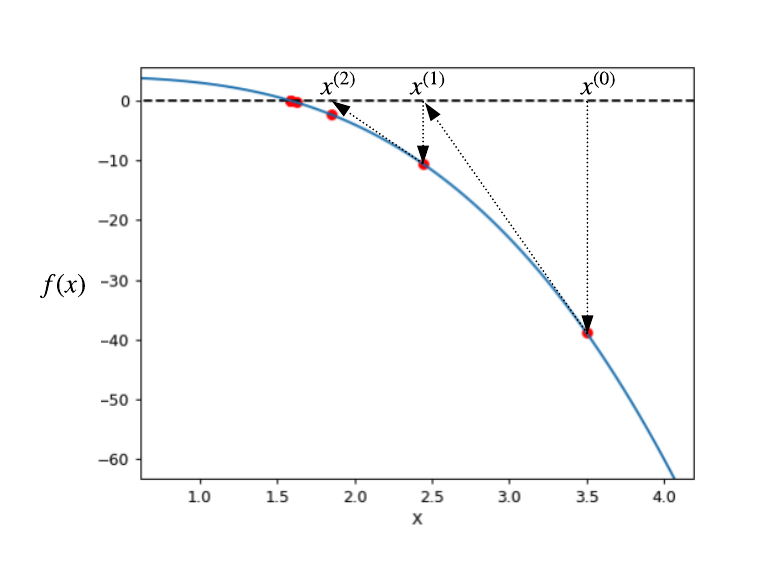
\includegraphics[width=\linewidth]{images/NR-1D.png}
    \end{center}
    \end{column}
    \begin{column}{0.45\textwidth}
    The \textit{convergence is quadratic} if we start with x(0) "close” to the solution.

    \href{https://colab.research.google.com/drive/12tCcO6kPxkoScAGnUYxgumS3CVSBSmtJ?usp=sharing}{\underline{Link to Python implementation}} 
    \end{column}
    \end{columns}
    
\end{frame}

\begin{frame}[allowframebreaks]{Newton-Raphson for the power flow problem}
    We apply exactly the same idea to our problem, except that we are in dimension $2 n_{PQ} + n_{PV}$.
    
    Hence we must compute partial derivatives to compute the update steps:
    $$\mathbf{\bar{V}}^{(i+1)}_x = \mathbf{\bar{V}}^{(i)}_x + \underbrace{\left[\mathbf{J}(\mathbf{\bar{V}}^{(i)})\right]^{-1} (\mathbf{F}^0-\mathbf{f}(\mathbf{\bar{V}}^{(i)}))}_{\Delta \mathbf{\bar{V}}_x}$$
    where
    \begin{itemize}
        \item $\mathbf{F}^0$ gathers the measured active powers at buses in $\mathcal{N}_{PQ} \cup \mathcal{N}_{PV}$ and reactive powers at buses $\mathcal{N}_{PQ}$
        \item $\mathbf{f}(\mathbf{\bar{V}})$ gathers the active and power flow equations at the corresponding buses
        \item $\mathbf{\bar{V}}_x$ is the subvector of $\mathbf{\bar{V}}$ that gathers the unknwon voltage magnitudes and angles at the the corresponding buses
        \item $\mathbf{J}(\mathbf{\bar{V}})$ is the jacobian of $\mathbf{f}$, of size $(2 n_{PQ} + n_{PV}) \times (2 n_{PQ} + n_{PV})$
    \end{itemize}

\end{frame}

\begin{frame}{Remarks}
    \begin{itemize}
        \item In practice, instead of computing the inverse of the Jacobian, we solve the system
        \begin{equation}
        \mathbf{J}(\mathbf{\bar{V}}^{(i)}) \Delta \mathbf{\bar{V}}_x = \mathbf{F}^0-\mathbf{f}(\mathbf{\bar{V}}^{(i)}) \label{eq:NR_step}
        \end{equation}
        to get the update step
        \item The Jacobian is often sparse, since a bus is connected to a few neighbors; it is very important to take into account the sparsity properties in practical implementations
        \item The Jacobian is not necessarily updated at every iteration, especially close to convergence
    \end{itemize}
\end{frame}

\begin{frame}[allowframebreaks]{Illustration}
Let's reconsider the 3-bus example we already modeled with PandaPower.

We will 
\begin{enumerate}
  \item Compute the line impedances of the system $Z_{1,2}, Z_{1,3}, Z_{2,3}$ where $Z_{i, j}$ is the impedance of the line between bus-$i$ and bus-$j$.
  \item Calculate the base impedance $Z_{B}$ and compute the per-unit line impedances.
  \item Compose the per-unit admittance matrix of the system $\mathbf{Y}_{p u} = \mathbf{G}_{p u} + j\mathbf{B}_{p u}$.
  \item Initialize the unknown voltages of the Newton-Raphson procedure:
  \begin{itemize}
    \item there are two unknowns at the PQ bus ($V_{3}, \theta_{3}$) and one unknown at the PV bus ( $\theta_{2}$ ).
    \item initialize the unknown magnitudes at 1 pu and unknown phases at 0 rad (first arbitrary estimation).
  \end{itemize}
  \item Perform one iteration in the Newton-Raphson procedure.
  \begin{itemize}
    \item Use the active and reactive power equations \eqref{eq:pf_P} and \eqref{eq:pf_Q} at the nodes where active and reactive power are known, i.e. estimate $p_2\left(\bar{V}^{(k)}\right), p_3\left(\bar{V}^{(k)}\right)$ and $q_3\left(\bar{V}^{(k)}\right)$, for $k=0$
    \item Compute the \textbf{error} of the initial step: subtract estimates from known values.
    \item Compute the Jacobian matrix $\mathbf{J}$ of the system and evaluate it at $\overline{\mathbf{V}}^{(0)}$.
    \item Find the \textbf{update step} $\Delta \overline{\mathbf{V}}$ by solving \eqref{eq:NR_step}.
    \item Update the estimated voltages magnitudes and phases with the \textbf{update step}
  \end{itemize}
  \item Repeat the process until the \textbf{error} is low enough.
\end{enumerate}
\begin{block}{Exercise}
    \begin{itemize}
    \item Write down the expression of $p_{2}\left(\bar{V}^{(k)}\right)$
    \item What are the dimensions of the Jacobian?
    \item Write down the expression of 3 elements of the Jacobian.
    \item Understand and run the \href{https://github.com/bcornelusse/ELEC0447-analysis-power-systems/tree/master/notebooks/power_flow_3-bus_Newton_Raphson.ipynb}{\underline{Python notebook}} 
    \textbf{WARNING: indices start at 0 in Python, so bus 1 is at index 0, etc.}
    \item Compare the results to the PandaPower model.
\end{itemize}

\end{block}


\end{frame}

\begin{frame}[allowframebreaks]{Fast decoupled power flow}
    Remember that
    \begin{itemize}
        \item active power flow is mostly a function of voltage angles
        \item reactive power flow is mostly a function of voltage magnitudes
    \end{itemize}
    
    If we apply these ideas stricly, we can subdivide the problem in two much simpler subproblems:
    \begin{itemize}
        \item one problem for angles, based on the active power measurements and the sub-Jacobian containing the partial derivatives of the active power flow equations w.r.t. angles
        \item one problem for magnitudes, based on the reactive power measurements and the sub-Jacobian containing the partial derivatives of the reactive power flow equations w.r.t. magnitudes
    \end{itemize}
    
    This procedure, through the sub-Jacobian that are computed, also provide information useful for \textit{sensitivity analysis}.
\end{frame}

\begin{frame}[allowframebreaks]{DC power flow}
    "Direct Current" power flow is a further simplification:
    \begin{itemize}
        \item it is assumed that the impact of the reactance of lines is much bigger than the impact of their resistance, and shunt conductances are neglected
        \item voltage magnitudes are assumed equal to $1 pu$
        \item angle differences are small
        \item active power losses are neglected, reactive power flows as well
    \end{itemize}
    
    $$P_k =  \sum_{m \in \mathcal{N} \setminus k} B_{km} \theta_{km}$$
    for every bus but the slack bus, which sets the angle difference, and collects the algebraic sum of all other injected powers.
    
    In matrix form, with $\mathbf{Y}$ the admittance matrix defined before:
    $$\mathbf{P} =  \Im(\mathbf{Y}) \mathbf{\theta}$$
    
    This is usefull for fast simulations, or when including a power flow model in an optimization problem, e.g. \href{https://bcornelusse.github.io/material/CoursEM20170331.pdf}{day-ahead market coupling}.
\end{frame}

\begin{frame}{Illustration of DC power flow}
    \begin{block}{Application to the 3-bus case}
        \begin{itemize}
            \item Show how to obtain the relaxation of the DC power flow
            \item Apply the DC approximation to the 3 bus case
            \item Understand the code and analyze the results: \href{https://github.com/bcornelusse/ELEC0447-analysis-power-systems/tree/master/notebooks/power_flow_3-bus_DC.ipynb}{\underline{Python notebook}}    
        \end{itemize}
    \end{block}
    
\end{frame}




%\bibliographystyle{ieeetr}
%\bibliography{demo}
%\end{frame}
%\begin{frame}[allowframebreaks]{References}

\end{document}

\begin{columns}
    \begin{column}{0.55\textwidth}

    \end{column}
    \begin{column}{0.45\textwidth}

    \end{column}
\end{columns}
